\documentclass[../../main/main.tex]{subfiles}
\graphicspath{{./figures/}}

\dominitoc
\faketableofcontents

\makeatletter
\renewcommand{\@chapapp}{\'Electrocin\'etique -- chapitre}
\makeatother

% \toggletrue{student}
% \HideSolutionstrue

\begin{document}
\setcounter{chapter}{2}

\chapter{Capacit\'es et inductances~: circuits du 1\ier{} ordre}

\vfill

\begin{prgm}
	\begin{tcb}*(ror)"know"{Savoirs}
		\begin{itemize}[label=$\diamond$, leftmargin=10pt]
			\item Connaître les relations entre l'intensité et la tension.
			\item Citer des ordres de grandeurs des composants $R$, $L$, $C$.
			\item Exprimer l'énergie stockée dans un condensateur ou une bobine.
			\item Distinguer, sur un relevé expérimental, régime transitoire et
			      régime permanent au cours de l'évolution d'un système du premier
			      ordre soumis à un échelon de tension.
			\item Interpréter et utiliser la continuité de la tension aux bornes d'un
			      condensateur ou de l'intensité du courant traversant une bobine.
		\end{itemize}
	\end{tcb}

	\begin{tcb}*(ror)"how"{Savoir-faire}
		\begin{itemize}[label=$\diamond$, leftmargin=10pt]
			\item Établir l'équation différentielle du premier ordre vérifiée par une
			      grandeur électrique dans un circuit comportant une ou deux mailles.
			\item Déterminer la réponse temporelle dans le cas d'un régime libre ou
			      d'un échelon de tension
			\item Déterminer un ordre de grandeur de la durée du régime transitoire.
			\item Réaliser un bilan énergétique.
		\end{itemize}
	\end{tcb}
\end{prgm}

\vfill
\minitoc
\vfill

\newpage

\section{Condensateur et circuit RC}
\subsection{Présentation du condensateur}
\subsubsection{Composition}

Après les résistances, les condensateurs sont les composants les plus répandus
en électronique. Le condensateur est un composant électronique couramment
utilisé dans les circuits les plus divers : microprocesseurs, mémoires, horloges électroniques, émetteurs et récepteurs radio, amplificateurs, etc.

\begin{tcb}[label=def:condens, sidebyside, righthand ratio=.3](defi){Condensateur}
	Un condensateur est un composant constitué de deux \textbf{surfaces
		conductrices}\footnote{Ce sont souvent des plaques, parfois des demi-sphères
		ou d'autres formes.} appelées \textit{armatures} et séparées par un
	\textbf{matériau isolant}\footnote{Par exemple l'air ou du polyéthylène.}.
	Son symbole est représenté ci-contre.
	\tcblower
	\begin{center}
		\switch{
			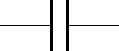
\includegraphics[width=.8\linewidth, draft=true]{condens_plain}
		}{
			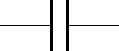
\includegraphics[width=.8\linewidth]{condens_plain}
		}
		\captionof{figure}{}
	\end{center}
\end{tcb}

\subsubsection{Relations fondamentales}
Quand un courant traverse le condensateur, des charges s'accumulent sur
les plaques~: si l'une est chargée $q$, l'autre est chargée $-q$.
\begin{tcb}[label=prop:Ccondens, sidebyside, righthand ratio=.3](prop){Charge et capacité}
	\begin{isd}[righthand ratio=.3, sidebyside align=top]
		La \textbf{tension à ses bornes} est \textbf{proportionnelle à $q$}, et on
		appelle ce coefficient de proportionnalité sa \textbf{capacité} notée $C$.
		On a donc
		\psw{
			\[\boxed{q = Cu}\]
		}
		\vspace*{-15pt}
		\tcblower
		\tcbsubtitle[before skip=\baselineskip,
			colback=red!80!black,
			colframe=red!80!black]{\fatbox{Unité}}
		\psw{
			$C$ en Farad (F)
		}
		\vspace{-15pt}
	\end{isd}
	\tcblower
	\begin{center}
		\switch{
			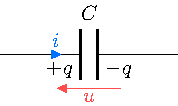
\includegraphics[width=.8\linewidth, draft=true]{condens_q}
		}{
			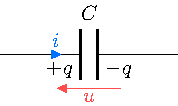
\includegraphics[width=.8\linewidth]{condens_q}
		}
		\captionof{figure}{}
	\end{center}
\end{tcb}

\begin{tcb}(odgr){Ordre de grandeur}
	Le Farad est une «~grande~» unité~: on trouvera des valeurs entre le \si{mF}
	(\SI{e-3}{F}) et le \si{pF} (\SI{e-12}{F})~:
	\begin{itemize}
		\item En électronique, on est entre le \si{nF} et le \si{\micro F}~;
		\item En électrotechnique, on est plutôt de l'ordre de \SI{10}{mF}~;
		\item Une capacité parasite est autour du \si{pF}.
	\end{itemize}
\end{tcb}

Pour caractériser le fonctionnement d'une capacité, on s'intéresse au lien entre
son courant et sa tension, comme on le fait pour une résistance ($U = RI$). On
remarque que~:
\begin{itemize}
	\item si $i > 0$, des charges arrivent sur l'armature de gauche, la charge
	      augmente donc la tension aussi~;
	\item si $i < 0$, des charges repartent, la charge diminue donc la tension
	      aussi~;
	\item si $i = 0$, aucune charge ne bouge, la quantité de charge sur
	      l'armature de gauche ne varie pas, la tension est constante.
\end{itemize}

Cette relation entre le \textbf{signe de $i$} et la \textbf{variation de $u$}
suggère que $i$ est relié à la dérivée de $u$. On a alors~:

\begin{tcbraster}[raster columns=2, raster equal height=rows]
	\begin{tcb}[label=prop:Ccarac](prop){Relation courant-tension}
		Pour un condensateur \textbf{en convention récepteur}, l'intensité que
		le traverse s'exprime par
		\psw{
			\[\boxed{i = C \dv{u_C}{t}}\]
		}
		\vspace{-15pt}
	\end{tcb}
	\begin{tcb}[label=demo:Ccarac](demo)'r'{Relation courant-tension}
		Par définition de $i$ et de la charge,
		\psw{
			\begin{DispWithArrows*}
				i & = \dv{q}{t}
				\Arrow{$q=Cu_C$}
				\\
				i & = C \dv{u_C}{t}
			\end{DispWithArrows*}
		}
		\vspace{-15pt}
	\end{tcb}
\end{tcbraster}

\subsubsection{Cas particuliers}

\begin{tcbraster}[raster columns=2, raster equal height=rows]
	\begin{tcb}[label=impl:continuité](impl){Continuité}
		Si $u_C$ présente une variation brusque, alors $ \dv{u_C}{t}$ devrait
		être infini. Or, comme $i = C \dv{u_C}{t}$, ceci n'est pas possible
		puisque ça impliquerait que le courant le soit. Ainsi,
		\begin{framed}
			\psw{
				La tension $u_C(t)$ aux bornes d'un condensateur ne peut pas
				varier instantanément, c'est une fonction continue.
			}
		\end{framed}
	\end{tcb}
	\begin{tcb}*[label=impl:permanent](impl)"limp"'r'{Régime permanent}
		En régime permanent (continu), les tensions et courants ne dépendent pas
		du temps. Alors $i = C \dv{u_C}{t} = 0$, ainsi
		\begin{framed}
			\psw{
				En régime permanent, le condensateur se comporte comme un
				interrupteur ouvert et bloque le courant.
			}
		\end{framed}
	\end{tcb}
\end{tcbraster}

\subsubsection{Associations}
\begin{tcbraster}[raster columns=2, raster equal height=rows]
	\begin{tcb}[label=prop:cserie](prop){Association en série}
		Deux condensateurs $C_1$ et $C_2$ en série forment un dipôle équivalent de
		capacité
		\psw{
			\[
				\boxed{\dfrac{1}{C_{\rm eq}} = \dfrac{1}{C_1} + \dfrac{1}{C_2}}
			\]
		}
		On dit qu'\textbf{en série, l'inverse des capacités s'ajoutent}.
		\tcblower
		\begin{center}
			\switch{
				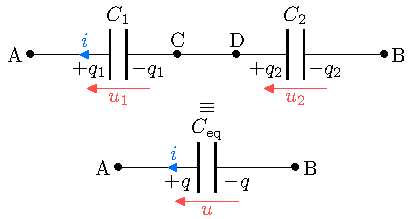
\includegraphics[width=\linewidth, draft=true]{cserie}
			}{
				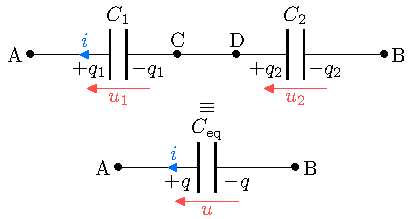
\includegraphics[width=\linewidth]{cserie}
			}
			\captionof{figure}{}
		\end{center}
	\end{tcb}
	\begin{tcb}[label=demo:cserie](demo)'r'{Association en série}
		\psw{
			Entre les deux condensateurs se situe un fil. Or, il n'y a pas de
			différence de potentiel sur un fil~: les deux points C et D sont au même
			potentiel. On déduit ainsi
			\begin{gather*}
				u_{CD} = u_{C} - u_{D} = 0 \Lra q_2 - q_1 = 0
				\\\Lra
				\boxed{q_2 = q_1 = q}
			\end{gather*}
			et les condensateurs en série portent la même charge $q$. Ainsi,
			\begin{DispWithArrows*}
				u & = u_1 + u_2
				\Arrow{$q=Cu$}
				\\\Lra
				u & = \frac{q}{C_1} + \frac{q}{C_2}
				\\\Lra
				u & = \left(\frac{1}{C_1} + \frac{1}{C_2}\right)q
			\end{DispWithArrows*}
			On a bien l'expression d'un unique condensateur de capacité
			\fbox{$\frac{1}{C_{\rm eq}} = \frac{1}{C_1} + \frac{1}{C_2}$}
		}
	\end{tcb}
\end{tcbraster}

\begin{tcbraster}[raster columns=2, raster equal height=rows]
	\begin{tcb}[label=prop:cpara](prop){Association en parallèle}
		Deux condensateurs $C_1$ et $C_2$ en dérivation forment un dipôle
		équivalent de capacité
		\psw{
			\[
				\boxed{C_{\rm eq} = C_1 + C_2}
			\]
		}
		On dit qu'\textbf{en parallèle, les capacités s'ajoutent}.
		\tcblower
		\begin{center}
			\switch{
				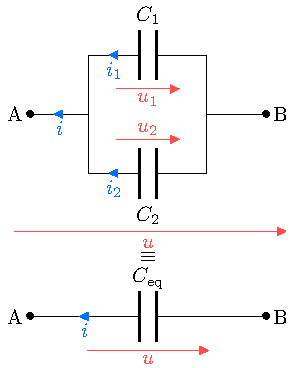
\includegraphics[width=.7\linewidth, draft=true]{cpara}
			}{
				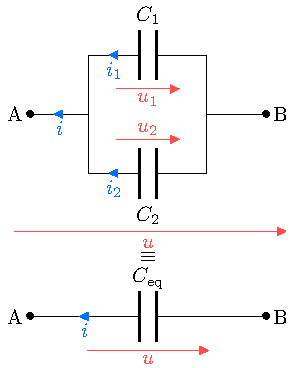
\includegraphics[width=.7\linewidth]{cpara}
			}
			\captionof{figure}{}
		\end{center}
	\end{tcb}
	\begin{tcb}[label=demo:cpara](demo)'r'{Association en parallèle}
		\psw{
			\[i = i_1+i_2\]
			On utilise ensuite la relation courant-tension~:
			\[
				C_{\rm eq} \dv{u}{t} = C_1 \dv{u}{t} + C_2 \dv{u}{t}
			\]
			On a bien l'expression d'un unique condensateur de capacité
			\[
				\boxed{C_{\rm eq} = C_1 + C_2}
			\]
		}
	\end{tcb}
\end{tcbraster}

\subsubsection{Condensateur réel}

\noindent
\begin{minipage}[t]{.69\linewidth}
	Dans la réalité, un condensateur possède des effets résistifs.
	Les deux armatures d'un condensateur réel sont séparés par un matériau
	qui conduit très légèrement le courant. Ainsi, un condensateur réel se
	modélise par un condensateur idéal en parallèle avec une résistance $R_f$,
	nommée résistance de fuite.
	\smallbreak
	L'ordre de grandeur de $R_f$ est de $\SI{e7}{\Omega}$
\end{minipage}
\hfill
\begin{minipage}[t]{.30\linewidth}
	~
	\vspace{-40pt}
	\begin{center}
		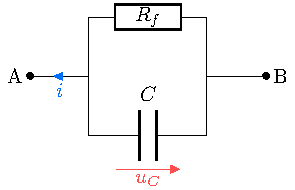
\includegraphics[width=\linewidth]{creel}
		\captionof{figure}{}
		\label{fig:creel}
	\end{center}
\end{minipage}

\subsubsection{Énergie stockée dans un condensateur}
\begin{tcb}(demo)<lfnt>{}
	\textbf{En convention récepteur}, la puissance \textbf{reçue} est
	\psw{
		\begin{DispWithArrows*}
			\Pc_{C} &= u_Ci
			\Arrow{$i = C \dv{u_C}{t}$}
			\\\Lra
			\Pc_{C} &= Cu_C \dv{u_C}{t} \triangleq \dv{\Ec_C}{t}
		\end{DispWithArrows*}
	}
	\vspace{-15pt}
	\leftcenters{\hspace{-12pt}Or, $\forall f$ fonction dérivable,}
	{\psw{$\DS\boxed{f\times f' = \left( \frac{1}{2}f^2 \right)'}$}}
	\smallbreak
	Ainsi,
	\psw{
		\[
			\Pc_{C} = \dv{t} \left( \frac{1}{2} Cu_C{}^2 \right)
			\Rightarrow \Ec_C(t) = \frac{1}{2}C u_C(t)^2
		\]
	}
	\vspace{-15pt}
\end{tcb}

\begin{tcb}[label=prop:Ec](prop){Énergie stockée dans un condensateur}
	\psw{
	\[
		\boxed{\Ec_C(t) = \frac{1}{2}C u_C{}^2(t)}
	\]
	}
	\vspace{-10pt}
\end{tcb}
\begin{tcb}[label=rema:genrec, sidebyside](rema){Condensateur récepteur ou
			générateur}
	Par l'étude de la relation précédente,
	\psw{
		\[
			u_C \nearrow \quad \Ra \dv{u_C}{t} > 0 \Rightarrow \Pc_{C} > 0
		\]
	}
	ainsi, le condensateur reçoit bien de l'énergie au reste du circuit, et il se
	\textbf{comporte comme récepteur}.
	\tcblower
	À l'inverse, on lit que
	\psw{
		\[
			u_C \searrow \quad \Ra \dv{u_C}{t} < 0 \Rightarrow \Pc_{C} < 0
		\]
	}
	ainsi, le condensateur cède en réalité de l'énergie au reste du circuit,
	autrement dit \textbf{il peut se comporter comme générateur}~!
\end{tcb}

\subsection{Circuit RC série~: charge}

On appelle \textbf{circuit linéaire du premier ordre} un circuit électrique
dont l'évolution des grandeurs électriques est régie par des équations
différentielles linéaires à coefficients constants et \textit{du premier
	ordre}. On étudie ici leur réponse à un échelon de tension.

\begin{tcb}[label=def:echelon, sidebyside, righthand ratio=.4](defi){Échelon de tension}
	Un échelon de tension est montant s'il est de la forme
	\[
		\left\{
		\begin{array}{rcl}
			u(t<0)    & = & 0 \\
			u(t\geq0) & = & E
		\end{array}
		\right.
	\]
	et descendant si $E$ avant et 0 après.
	\tcblower
	\begin{center}
		\switch{
			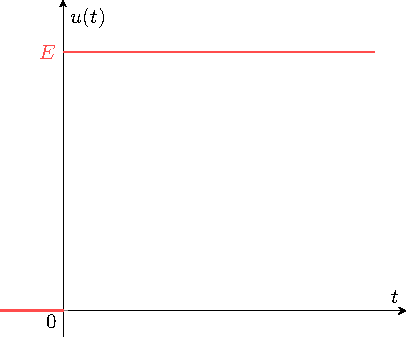
\includegraphics[width=\linewidth, draft=true]{echelon}
		}{
			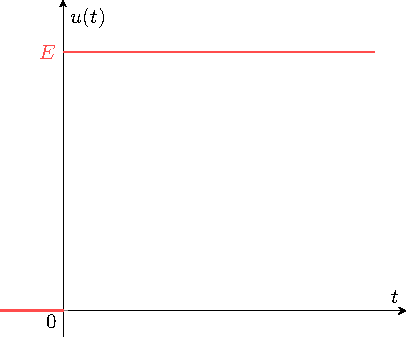
\includegraphics[width=\linewidth]{echelon}
		}
		\captionof{figure}{}
	\end{center}
\end{tcb}

\subsubsection{Présentation}
\noindent
\begin{minipage}[c]{.6\linewidth}
	\begin{itemize}
		\item Il est constitué d'un générateur idéal de tension en série avec une
		      résistance et un condensateur idéal.
		\item \textbf{On suppose le condensateur initialement déchargé}.
		\item À $t=0$, on ferme l'interrupteur.
	\end{itemize}
\end{minipage}
\hfill
\begin{minipage}[c]{.35\linewidth}
	~
	\begin{center}
		\switch{
			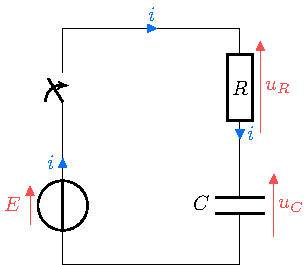
\includegraphics[width=.9\linewidth, draft=true]{circ_rc-start}
		}{
			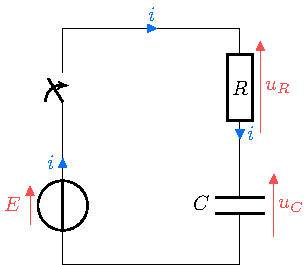
\includegraphics[width=.9\linewidth]{circ_rc-start}
		}
		\label{fig:circ_rc-start}
		\captionof{figure}{}
	\end{center}
\end{minipage}

\subsubsection{Équation différentielle du circuit}
On cherche à connaître la tension aux bornes du condensateur à partir du moment
où l’on ferme l’interrupteur, soit à $t \geq 0$.
\begin{tcb}[label=demo:eqdiffrc](demo)<lfnt>{Équa. diff. RC montant}
	Avec la loi des mailles,
	\psw{
		\begin{DispWithArrows*}
			u_R + u_C &= E
			\Arrow{$u_R = Ri$\\et $i = C \dv{u_C}{t}$}
			\\\Lra
			RC \dv{u_C}{t} + u_C        & = E
			\\\Lra
			\dv{u_C}{t} + \frac{1}{RC}u_C & = \frac{E}{RC}
		\end{DispWithArrows*}
	}
	\vspace{-15pt}
\end{tcb}
\begin{tcb}[label=prop:eqdiffrc, sidebyside, righthand ratio=.4](prop){Équation
			différentielle RC échelon montant}

	L'équation différentielle de la tension $u_C(t)$ aux bornes d'un condensateur
	dans un circuit RC avec un échelon de tension montant $E$ s'écrit
	\psw{
		\[
			\boxed{\dv{u_C}{t} + \frac{1}{\tau}u_C = \frac{E}{\tau}}
		\]
	}
	avec \fbox{$\tau = RC$} la constante de temps.
	\tcblower
	C'est une équation différentielle linéaire du premier ordre à
	coefficients et second membre constants, de condition initiale
	\psw{
		\[
			\boxed{u_C(0^-) = u_C(0^+) = 0}
		\]
	}
\end{tcb}

\begin{tcb}(appl){Dimension de $RC$}
	Montrer, par analyse dimensionnelle, que $RC$ est homogène à un temps.
	\tcblower
	\begin{isd}[sidebyside align=top]
		\tcbsubtitle{\fatbox{Méthode 1}}
		\psw{
			On a $[RC] = \si{\Omega.F}$. Or,
			\begin{align*}
				[q] = [Cu] & \Lra \si{C} = \si{F.V}
				\\
				           & \Lra \si{F} = \si{C.V^{-1}}
				\\
				           & \Lra \si{F} = \si{A.s.V^{-1}}
			\end{align*}
			de plus,
			\begin{align*}
				[u] = [Ri] & \Lra \si{V} = \si{\Omega.A}
				\\
				           & \Lra \si{\Omega} = \si{V.A^{-1}}
			\end{align*}
			Ainsi,
			\begin{align*}
				[RC]         & = \si{\Omega.F}
				\\\Lra
				[RC]         & = \si{V.A^{-1}.A.s.V^{-1}}
				\\\Lra
				\Aboxed{[RC] & = \si{s}}
				\qed
			\end{align*}
		}
		\tcblower
		\tcbsubtitle{\fatbox{Méthode 2}}
		\psw{
			Une équation physique étant homogène, comme
			\[
				\dv{u_C}{t} + \frac{u_C}{RC} = \frac{E}{RC}
			\]
			alors
			\begin{align*}
				\left[ \dv{u_C}{t} \right] & = \left[\frac{u_C}{RC}\right]
				\\\Lra
				\frac{[u_C]}{[t]}          & = \frac{[u_C]}{[RC]}
				\\\Lra
				\Aboxed{[RC]               & = [t]}
				\qed
			\end{align*}
		}
	\end{isd}
\end{tcb}

\subsubsection{Résolution de l'équation différentielle}
\begin{tcb}[label=impo:eqres, heart](ror){Résolution équation différentielle
			coefficients constants}
	Pour résoudre une équation différentielle linéaire à
	coefficients constants et second membre constant, de la forme
	$\DS \dv{y}{y} + \frac{1}{\tau}y = k$~:
	\begin{enumerate}[label=\sqenumi]
		\item On écrit l'\textbf{équation homogène} associée à
		      l'équation différentielle obtenue.
		\item On écrit la \textbf{forme générale de la solution de
			      l'équation homogène}.
		\item On recherche une \textbf{solution particulière
			      constante de l'équation générale}, de la forme $y(t) =
			      \lambda$.
		\item On écrit la \textbf{solution générale}, somme de la
		      solution particulière et de la forme générale.
		\item On détermine la constante à l'aide des
		      \textbf{conditions initiales}.
	\end{enumerate}
\end{tcb}
\begin{tcb}[label=demo:rcsolu](demo){Solution RC série montant}
	\begin{enumerate}[label=\sqenumi]
		\item L'équation homogène est~:
		      \psw{
			      \[
				      \dv{u_C}{t} + \frac{1}{\tau}u_C = 0
			      \]
		      }
		      \vspace{-15pt}
		\item La forme générale de la solution pour cette équation est~:
		      \psw{
			      \[
				      u_C(t) = K\exp\left( -\frac{t}{\tau} \right)
			      \]
		      }
		      \vspace{-15pt}
		\item Une solution particulière avec $u_C(t) = \lambda$ donne
		      \psw{
			      \[
				      0 + \frac{\lambda}{\tau} = \frac{E}{\tau}
			      \]
			      Donc $u_C(t) = E$ est \textbf{une} solution de l'équation
			      différentielle.
		      }
		\item La solution générale est donc
		      \psw{
			      \[
				      u_C(t) = E + K\exp \left( - \frac{t}{\tau} \right)
			      \]
		      }
		      \vspace{-15pt}
		\item Les conditions initiales donnent ici
		      \[
			      \psw{u_C(t=0) = 0}
			      \qqet
			      \psw{u_C(0) = K + E \Ra K=-E}
		      \]
	\end{enumerate}
\end{tcb}
\begin{tcb}[label=prop:ucsolu, sidebyside, righthand ratio=.4](prop){Solution
			de l'équation différentielle RC montant}
	La solution de l'équation différentielle de la tension $u_C(t)$
	d'un circuit RC soumis à un échelon de tension $E$ avec
	$u_C(0) = 0$ est
	\psw{
		\[
			\boxed{u_C(t) = E\left(1-\exp\left(-\frac{t}{\tau}\right)\right)}
		\]
	}
	\vspace{-15pt}
	\tcblower
	\begin{center}
		\switch{
			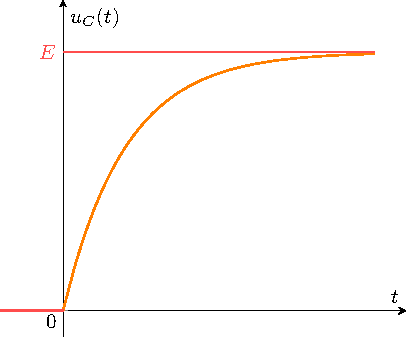
\includegraphics[width=\linewidth, draft=true]{carac_rc}
		}{
			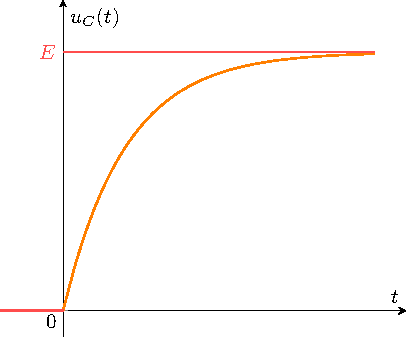
\includegraphics[width=\linewidth]{carac_rc}
		}
		\captionof{figure}{}
	\end{center}
\end{tcb}

\subsubsection{Constante de temps, régime transitoire}
Quand $t \ra +\infty$, $u_C(t) = E$. On est alors en \textbf{régime permanent}~:
$u_C(t)$ ne varie plus. La vitesse à laquelle ce régime est atteint dépend de la
valeur de $\tau$ la constante de temps. On détaille ici comment la déterminer~:
\begin{tcbraster}[raster columns=2, raster equal height=rows]
	\begin{tcb}[label=impl:déterm](exem){Détermination $\tau$}
		Avec la courbe $u_C(t)$, on remarque que~:
		\begin{enumerate}
			\item \psw{
				      $u_C(\tau) = E \left( 1-e^{-1} \right) \approx
					      \num{0.632}\times E$
			      }
			      \smallbreak
			      Donc on trouve $\tau$ en lisant l'abscisse telle que $u_C(\tau) =
				      \num{0.632}\times E$.
			\item En $t=0$, l'équation différentielle donne
			      \psw{
				      \[
					      \dv{u_C}{t}\/ (0) + \underbracket[1pt]{\frac{u_C(0)}{\tau}}_{=0}
					      = \frac{E}{\tau}
				      \]
			      }
			      La tangente à la courbe en 0, de pente $\frac{E}{\tau}$ coupe donc
			      l'asymptote en $t = \tau$.
		\end{enumerate}
	\end{tcb}
	\begin{tcb}*[label=impl:tauRC](impl)"limp"'r'{Constante de temps}
		\switch{
			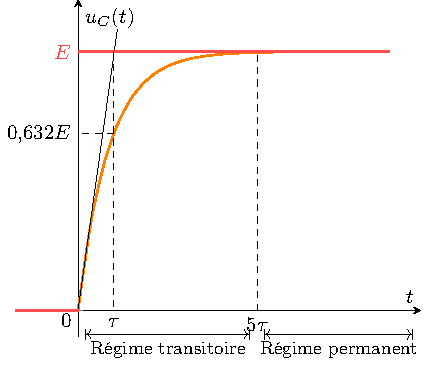
\includegraphics[width=\linewidth, draft=true]{carac_rc-tau}
		}{
			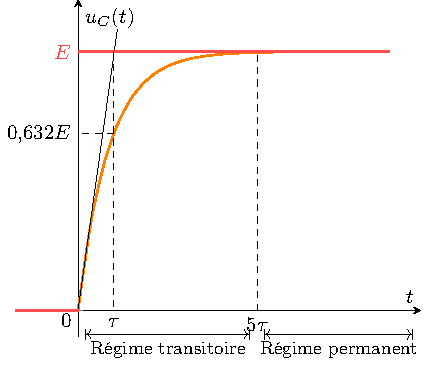
\includegraphics[width=\linewidth]{carac_rc-tau}
		}
		\captionof{figure}{}
	\end{tcb}
\end{tcbraster}
On distingue alors deux zones sur la courbe, approximativement séparées~: le
régime \textit{transitoire} et le régime \textit{permanent}. On cherche à
trouver au bout de combien de temps on peut considérer le régime permanent
atteint.
\smallbreak
Pour cela, on se fixe un \textbf{seuil arbitraire} à partir duquel on considère
le régime permanent atteint. Dans ce cours, on prendra $99\%$. On cherche donc
$t_{99}$ tel que $u(t_{99}) = \num{0.99}E$~:
\begin{tcb}(demo)<lfnt>{}
	\psw{
		\begin{DispWithArrows*}
			u_C(t_{99}) &= \num{0.99}E
			\Arrow{on utilise la solution de $u_C$}
			\\\Lra
			E\left(1-\exp(-\frac{t_{99}}{\tau})\right) &= \num{0.99}E
			\CArrow{$\mdiv E$}
			\\\Lra
			1 - \exp\left( -\frac{t_{99}}{\tau} \right) &= \num{0.99}
			\Arrow{on isole l'exp}
			\\\Lra
			\exp\left( -\frac{t_{99}}{\tau} \right) &= \num{0.01}
			\CArrow{$\ln (~)$}
			\\\Lra
			-\frac{t_{99}}{\tau} &= \ln (\num{0.01}) = -\ln (100)
			\Arrow{on isole $t_{99}$}
			\\\Lra
			\Aboxed{t_{99} &= \tau \ln (100)}
		\end{DispWithArrows*}
	}
	\vspace{-15pt}
\end{tcb}

\begin{tcb}(prop){Temps de réponse}
	\leftcenters{Ainsi,}
	{\psw{\fbox{le temps de réponse à 99\% est à \num{4.6}$\tau$}}}
\end{tcb}

\subsubsection{Évolution de l'intensité}
Qu'advient-il de l'intensité dans un circuit RC~? On peut le déterminer de deux
manières~:
\begin{tcb}[label=demo:irc-charge](demo)<lfnt>{Intensité RC charge}
	\begin{enumerate}
		\item Avec la caractéristique de C~:
		      \psw{
			      \begin{DispWithArrows*}
				      i(t)             & = C\DS \dv{u_C}{t}
				      \Arrow{$u_C(t) = E(1-\exr^{-t/\tau})$}
				      \\\Ra
				      i(t) & = CE \left(
				      0 - \left(-\frac{1}{\tau} \right)
				      \exp \left(- \frac{t}{\tau} \right)
				      \right)
				      \Arrow{$\tau = RC \Lra C/\tau = 1/R$}
				      \\\Lra
				      \Aboxed{i(t) &= \frac{E}{R}\exp \left(-\frac{t}{\tau} \right)}
			      \end{DispWithArrows*}
		      }
		\item Avec la loi des mailles~:
		      \psw{
			      \begin{DispWithArrows*}
				      Ri &= E-u_C
				      \Arrow{$u_C(t) = E(1-\exr^{-t/\tau})$}
				      \\\Lra
				      Ri(t) &= \cancel{E-E}+E \exp(-\frac{t}{\tau})
				      \CArrow{$\mdiv R$}
				      \\\Lra
				      \Aboxed{i(t) &= \frac{E}{R}\exp \left(-\frac{t}{\tau} \right)}
			      \end{DispWithArrows*}
		      }
	\end{enumerate}
\end{tcb}
\begin{tcb}[label=prop:irc-charge, sidebyside, righthand ratio=.4](prop){Intensité RC charge}
	L'intensité dans un circuit RC en charge s'exprime par
	\psw{
		\[
			\boxed{i(t) = \frac{E}{R}\exp \left(-\frac{t}{\tau} \right)}
		\]
	}
	\tcblower
	\begin{center}
		\switch{
			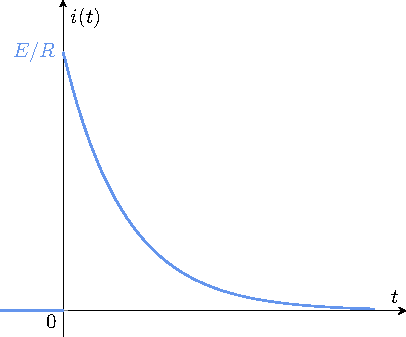
\includegraphics[width=\linewidth, draft=true]{carac_rcI}
		}{
			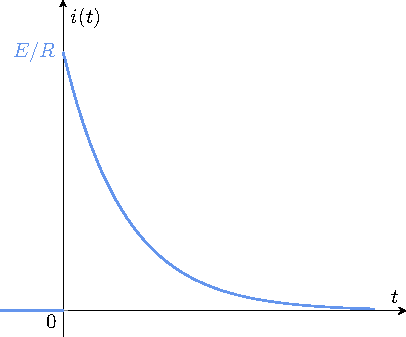
\includegraphics[width=\linewidth]{carac_rcI}
		}
		\captionof{figure}{}
	\end{center}
\end{tcb}

\subsubsection{Bilan de puissance}

En électrocinétique, les puissances sont le produit d'une tension et d'une
intensité. Or, par construction la loi des mailles est une relation entre les
tensions du circuit. Si on veut effectuer un bilan de puissance, on retiendra~:

\begin{tcb}[fontupper=\Large, bld, cnt](ror){Bilan de puissance en élec}
	On effectue un bilan de puissance en écrivant la loi des mailles multipliée
	par $i$.
\end{tcb}
\begin{tcb}[label=demo:rcpuiss-charge](demo)<lfnt>{Bilan de puissances}
	\vspace{-15pt}
	\psw{
		\begin{DispWithArrows*}
			u_C + Ri &= E
			\CArrow{$\times i$}
			\\\Lra
			u_C\,i + Ri^{2} &= Ei
			\Arrow{RCT pour C~: $i = C \dv{u_C}{t}$}
			\\\Lra
			u_C\,C \dv{u_C}{t} + Ri^{2} &= Ei
			\Arrow{$f \times f' = \left( \frac{1}{2}f^{2} \right)'$}
			\\\Lra
			\underbracket[1pt]{\dv{t} \left( \frac{1}{2}Cu_C{}^{2} \right)}
			_{\dv{\Ec_C}{t}} +
			\underbracket[1pt]{\vphantom{\dv{t} \left( \frac{1}{2}Cu_C{}^{2} \right)}
				Ri^{2}}_{\Pc_J}
			&=
			\underbracket[1pt]{\vphantom{\dv{t} \left( \frac{1}{2}Cu_C{}^{2} \right)}
				Ei}_{\Pc_G}
		\end{DispWithArrows*}
	}
	\vspace{-15pt}
\end{tcb}
\begin{tcb}[label=prop:rcpuiss-charge](prop){Bilan de puissances}
	Dans un circuit RC en charge, on a le bilan de puissances
	\psw{
		\[
			\boxed{\Pc_G = \Pc_C + \Pc_J}
		\]
	}
	\vspace{-15pt}
	\begin{itemize}[leftmargin=50pt]
		\item[$\Pc_G = Ei$] : \psw{
				la puissance fournie par le générateur~;
			}
		\item[$\Pc_C = \dv{\Ec_C}{t}$] : \psw{
				la puissance reçue par le condensateur~;
			}
		\item[$\Pc_J = Ri^{2}$] : \psw{
				la puissance dissipée par effet \textsc{Joule} dans la
				résistance.
			}
	\end{itemize}
\end{tcb}

\subsubsection{Bilan d'énergie}
On peut étudier énergétiquement cette évolution en intégrant la puissance
délivrée sur le temps d'utilisation. En effet, comme vu précédemment, $i(t)$
tend vers $0$ en $+\infty$, donc la puissance finale sera nulle et l'énergie
finie.
\begin{tcb}[label=demo:rcenerg-charge](demo)<lfnt>{Bilan d'énergie}
	L'énergie fournie par le générateur sur toute la charge est
	\psw{
		\begin{DispWithArrows*}[groups]
			\Ec_G &= \int_{0}^{+\infty} \Pc_G \dd t
			\Arrow{$\Pc_G = Ei$}
			\\
			&= \int_{0}^{+\infty} Ei(t) \dd t
			\Arrow{$i(t) = E/R \exr^{-t/\tau}$}
			\\
			&=
			\frac{E^2}{R} \left[
				-\tau \exp \left(-\frac{t}{\tau} \right)
				\right]_0^{+\infty}
			\\
			&=
			\frac{E^{2}}{R}
			\left(
			-\tau \underbracket[1pt]{\exp\left(-\frac{\infty}{\tau}\right)}_{=0}
			- \left( -\tau
				\xunderbracket{\exp(0)}_{=1}
				\right)
			\right)
			\\\Lra
			\Ec_G &= \tau \frac{E^2}{R}
			\Arrow{$\tau = RC$}
			\\\Lra
			\Aboxed{\Ec_G &= CE^2}
		\end{DispWithArrows*}
	}
	Or, l'énergie stockée dans le condensateur (propriété \ref{prop:Ec}) est
	\psw{
		\[
			\Ec_C = \frac{1}{2}CE^2
		\]
	}
	ainsi
	\psw{
		\[
			\Ec_J = \frac{1}{2}CE^2
		\]
	}
	\vspace{-15pt}
\end{tcb}
\begin{tcb}[label=prop:rcenerg-charge](prop){Bilan d'énergie}
	Pendant la totalité de la charge, l'énergie du générateur est
	\psw{
		\[\boxed{\Ec_G = CE^2}\]
	}
	Elle se répartit équitablement entre le condensateur et la résistance~:
	\psw{
		\[\boxed{\Ec_C = \frac{1}{2} CE^2 = \Ec_J}\]
	}
	\vspace{-15pt}
\end{tcb}

\subsection{Circuit RC série~: décharge}
\subsubsection{Présentation}
\noindent
\begin{minipage}[c]{.6\linewidth}
	\begin{itemize}
		\item Il est constitué d'un générateur idéal de tension en série avec une
		      résistance et un condensateur idéal.
		\item \textbf{On suppose le condensateur initialement chargé}~: $u_C(0^-) =
			      E$.
		\item À $t=0$, on coupe le générateur.
	\end{itemize}
	On dit que le système est \textbf{en régime libre} et soumis à un
	\textbf{échelon de tension descendant}.
\end{minipage}
\hfill
\begin{minipage}[c]{.35\linewidth}
	~
	\begin{center}
		\switch{
			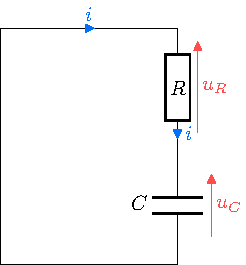
\includegraphics[width=.9\linewidth, draft=true]{circ_rc-decharge}
		}{
			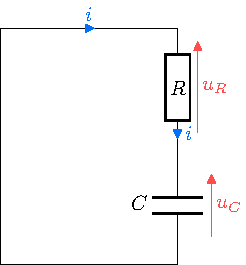
\includegraphics[width=.9\linewidth]{circ_rc-decharge}
		}
		\label{fig:circ_rc-start}
		\captionof{figure}{}
	\end{center}
\end{minipage}

\subsubsection{Équation différentielle du circuit}
\begin{tcbraster}[raster columns=2, raster equal height=rows]
	\begin{tcb}[label=prop:eqdiffrc](prop){Équa. diff. RC libre}
		L'équation différentielle de la tension $u_C(t)$ aux bornes d'un
		condensateur dans un circuit RC en décharge
		\psw{
			\[ \boxed{\dv{u_C}{t} + \frac{1}{\tau}u_C = 0}\]
		}
		avec \fbox{$\tau = RC$} la constante de temps.
		\tcblower
		C'est une équation différentielle linéaire du premier ordre à
		coefficients constants sans second membre, de condition initiale
		\psw{
			\[ \boxed{u_C(0^-) = u_C(0^+) = E}\]
		}
	\end{tcb}
	\begin{tcb}[label=demo:eqdiffrc](demo)'r'{Équa. diff. RC libre}
		Avec la loi des mailles,
		\psw{
			\begin{DispWithArrows*}[fleqn, mathindent=1cm]
				u_R + u_C &= 0
				\Arrow{$u_R = Ri$\\et $i = C \dv{u_C}{t}$}
				\\\Lra
				RC \dv{u_C}{t} + u_C        & = 0
				\\\Lra
				\dv{u_C}{t} + \frac{1}{RC}u_C & = 0
			\end{DispWithArrows*}
		}
	\end{tcb}
\end{tcbraster}

\subsubsection{Résolution de l'équation différentielle}
\begin{tcbraster}[raster columns=2, raster equal height=rows]
	\begin{tcb}[label=prop:ucsolu](prop){Solution équa. diff. RC libre}
		La solution de l'équation différentielle de la tension $u_C(t)$
		d'un circuit RC en décharge avec $u_C(0) = E$ est
		\psw{
			\[\boxed{u_C(t) = E\exp\left(-\frac{t}{\tau}\right)}\]
		}
	\end{tcb}
	\begin{tcb}[label=demo:rcsolu](demo)'r'{Solution équa. diff. RC libre}
		L'équation étant déjà homogène, on écrit la forme générale~:
		\psw{
			\[u_C(t) = K\exp\left( -\frac{t}{\tau} \right)\]
		}
		et on trouve $K$ avec la condition initiale~:
		\[
			\psw{u_C(0) = E}
			\qqet
			\psw{u_C(0) = K \Ra K=E}
		\]
	\end{tcb}
\end{tcbraster}

\subsubsection{Représentation graphique, constante de temps et transitoire}
\begin{tcbraster}[raster columns=2, raster equal height=rows]
	\begin{tcb}[label=impl:déterm](exem){Détermination $\tau$}
		\begin{enumerate}
			\item \psw{
				      $u_C(\tau) = E e^{-1} \approx \num{0.368}\times E$
			      }
			      \smallbreak
			      Donc on trouve $\tau$ en lisant l'abscisse telle que $u_C(\tau) =
				      \num{0.368}\times E$.
			\item En $t=0$, l'équation différentielle donne
			      \psw{
				      \[
					      \dv{u_C}{t}\/ (0) + \overbracket[1pt]{\frac{u_C(0)}{RC}}^{=E} = 0
				      \]
			      }
			      La tangente à la courbe en 0, de pente $-E/\tau$ coupe donc
			      l'asymptote en $t = \tau$.
		\end{enumerate}
	\end{tcb}
	\begin{tcb}*[label=impl:tauRC](impl)"limp"'r'{Constante de temps}
		\switch{
			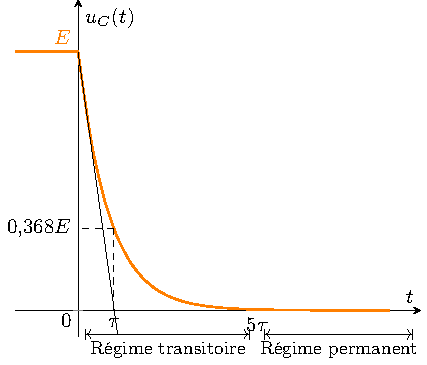
\includegraphics[width=\linewidth, draft=true]{carac_rc-tau_decharge}
		}{
			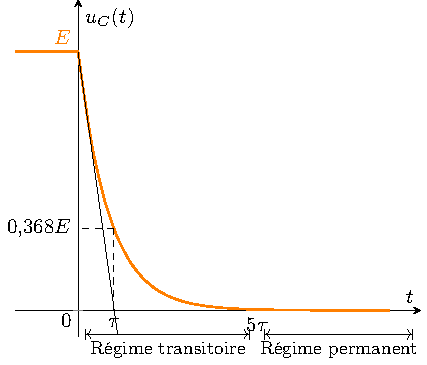
\includegraphics[width=\linewidth]{carac_rc-tau_decharge}
		}
		\captionof{figure}{}
	\end{tcb}
\end{tcbraster}
Comme précédemment, avec $t_{99}$ tel que $u_C(t_{99}) = \num{0.01}E$, on
trouve $t_{99} = \num{4.6}\tau$.
\begin{tcb}(prop){Temps de réponse}
	\leftcenters{Ainsi,}
	{\psw{\fbox{le temps de réponse à 99\% est à \num{4.6}$\tau$}}}
\end{tcb}

\subsubsection{Évolution de l'intensité}
\begin{tcb}[label=demo:irc-charge](demo)<lfnt>{Intensité RC décharge}
	\begin{enumerate}
		\item Avec la caractéristique de C~:
		      \psw{
			      \begin{DispWithArrows*}
				      i(t)             & = C\DS \dv{u_C}{t}
				      \Arrow{$u_C(t) = E\exr^{-t/\tau}$}
				      \\\Ra
				      i(t) & = - \frac{CE}{\tau} \exp \left(- \frac{t}{\tau} \right)
				      \Arrow{$\tau = RC \Lra C/\tau = 1/R$}
				      \\\Lra
				      \Aboxed{i(t) &= -\frac{E}{R}\exp \left(-\frac{t}{\tau} \right)}
			      \end{DispWithArrows*}
		      }
		\item Avec la loi des mailles~:
		      \psw{
			      \begin{DispWithArrows*}
				      Ri &= -u_C
				      \Arrow{$u_C(t) = E\exr^{-t/\tau}$}
				      \\\Lra
				      Ri(t) &= -E \exp(-\frac{t}{\tau})
				      \CArrow{$\mdiv R$}
				      \\\Lra
				      \Aboxed{i(t) &= -\frac{E}{R}\exp \left(-\frac{t}{\tau} \right)}
			      \end{DispWithArrows*}
		      }
	\end{enumerate}
\end{tcb}
\begin{tcb}[label=prop:irc-charge, sidebyside, righthand ratio=.4](prop){Intensité RC décharge}
	L'intensité dans un circuit RC en décharge s'exprime par
	\psw{
		\[
			\boxed{i(t) = -\frac{E}{R}\exp \left(-\frac{t}{\tau} \right)}
		\]
	}
	\tcblower
	\begin{center}
		\switch{
			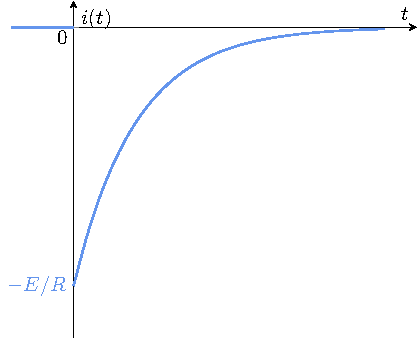
\includegraphics[width=\linewidth, draft=true]{carac_rcI-decharge}
		}{
			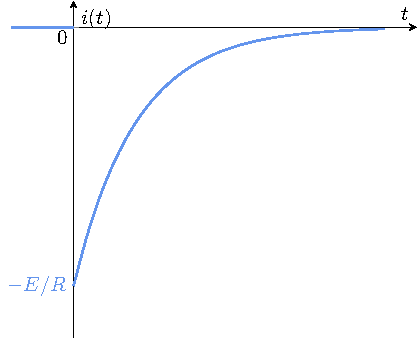
\includegraphics[width=\linewidth]{carac_rcI-decharge}
		}
		\captionof{figure}{}
	\end{center}
\end{tcb}

\subsection{Méthode pour les circuits à plusieurs mailles}
En général, les circuits étudiés sont constitués de plus d'une maille. Pour les
résoudre, on procède comme suit~:
\begin{tcb}(ror){Méthode avec plusieurs mailles}
	\begin{enumerate}[label=\sqenumi]
		\item Écrire les différentes lois du circuit (LdN, LdM, Ld$\Omega$, RCT…)~;
		\item Écrire les lois des mailles~;
		\item Isoler la grandeur dont on veut l'équation différentielle en éliminant
		      les autres~;
		\item mettre l'équation sous forme canonique~:
		      \[
			      \dv{f}{t} + \frac{f}{\tau} = \frac{F}{\tau}
		      \]
		      et identifier $F$ et $\tau$~;
		\item Établir les conditions initiales avec l'énoncé et la continuité de la
		      tension pour $C$~;
		\item Résoudre l'équation différentielle.
	\end{enumerate}

\end{tcb}


\section{Bobine et circuit RL}
\subsection{Présentation de la bobine}
\subsubsection{Composition}

Les bobines sont fréquemment utilisées dans les applications électrotechniques
(moteurs électriques, transformateurs). Comme elles sont lourdes et
encombrantes, elles sont plus rares en électronique.

\begin{tcb}[label=def:bobine, sidebyside, righthand ratio=.3](defi){Bobine}
	Une bobine est constituée de l'enroulement régulier d'une grande
	longueur d'un fil métallique, recouvert d'une gaine ou d'un vernis
	isolant. Son symbole est représenté ci-contre.
	\tcblower
	\begin{center}
		\switch{
			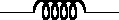
\includegraphics[width=.8\linewidth, draft=true]{bobine_plain}
		}{
			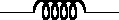
\includegraphics[width=.8\linewidth]{bobine_plain}
		}
		\captionof{figure}{}
	\end{center}
\end{tcb}

\subsubsection{Relation courant-tension}

\begin{tcb}[label=prop:Lcarac, sidebyside, righthand ratio=.3](prop){Relation courant-tension}
	\begin{isd}[righthand ratio=.3, sidebyside align=top]
		Quand un courant traverse la bobine, une tension apparaît à ses bornes.
		\textbf{En convention récepteur}, celle-ci s'exprime par
		\psw{
			\[\boxed{u_L = L\dv{i}{t}}\]
		}
		\tcblower
		on appelle $L$ l'\textbf{inductance} de la bobine.
		\tcbsubtitle{\fatbox{Unité}}
		\psw{
			$L$ en Henry (H)
		}
	\end{isd}
	\tcblower
	\begin{center}
		\switch{
			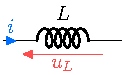
\includegraphics[width=.8\linewidth, draft=true]{bobine_u}
		}{
			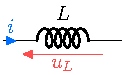
\includegraphics[width=.8\linewidth]{bobine_u}
		}
		\captionof{figure}{}
	\end{center}
\end{tcb}

\begin{tcb}(odgr){Ordre de grandeur}
	Le Henry est également un peu grande comme unité~: on trouvera des valeurs
	entre le \si{H} et le \si{\micro H} (\SI{e-6}{H}).
\end{tcb}

\subsubsection{Cas particuliers}

\begin{tcbraster}[raster columns=2, raster equal height=rows]
	\begin{tcb}[label=impl:continuité](impl){Continuité}
		Si $i$ présente une variation brusque, alors $ \dv{i}{t}$ devrait
		être infini. Or, comme $u_L = L\dv{i}{t}$, ceci n'est pas possible
		puisque ça impliquerait que la tension le soit. Ainsi,\vspace*{-10pt}
		\begin{framed}
			\psw{
				Le courant $i$ traversant une bobine ne peut pas
				varier instantanément, c'est une fonction continue.
			}
		\end{framed}
	\end{tcb}
	\begin{tcb}*[label=impl:permanent](impl)"limp"'r'{Régime permanent}
		En régime permanent (continu), les tensions et courants ne dépendent pas
		du temps. Alors $u_L = L \dv{i}{t} = 0$, ainsi
		\begin{framed}
			\psw{
				En régime permanent, la bobine se comporte comme un
				fil et la tension à ses bornes est nulle
			}
		\end{framed}
	\end{tcb}
\end{tcbraster}

\subsubsection{Associations}
\begin{tcb}[label=prop:bserie, sidebyside, righthand ratio=.3](prop){Association en série}
	Deux bobines $L_1$ et $L_2$ en série forment un dipôle équivalent
	d'inductance
	\psw{
		\[
			\boxed{L_{\rm eq} = L_1 + L_2}
		\]
	}
	On dit qu'\textbf{en série, les inductances s'ajoutent}.
	\tcblower
	\begin{center}
		\switch{
			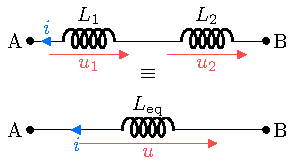
\includegraphics[width=\linewidth, draft=true]{bserie}
		}{
			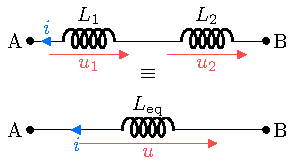
\includegraphics[width=\linewidth]{bserie}
		}
		\captionof{figure}{}
	\end{center}
\end{tcb}
\begin{tcb}[label=demo:bserie](demo)'r'{Association en série}
	\psw{
		\vspace{-15pt}
		\begin{DispWithArrows*}
			u & = u_1 + u_2
			\Arrow{$u_L = L \dv{i}{t}$}
			\\\Lra
			L_{\rm eq} \dv{i}{t} & = L_{1} \dv{i}{t} + L_{2} \dv{i}{t}
		\end{DispWithArrows*}
		On a bien l'expression d'une unique bobines d'inductance
		$\boxed{L_{\rm eq} = L_1 + L_2}$
	}
\end{tcb}

\begin{tcbraster}[raster columns=2, raster equal height=rows]
	\begin{tcb}[label=prop:bpara](prop){Association en parallèle}
		Deux bobines $L_1$ et $L_2$ en dérivation forment un dipôle
		équivalent d'inductance
		\psw{
			\[
				\boxed{\dfrac{1}{L_{\rm eq}} = \dfrac{1}{L_1} + \dfrac{1}{L_2}}
			\]
		}
		On dit qu'\textbf{en parallèle, l'inverse des inductances s'ajoutent}.
		\tcblower
		\begin{center}
			\switch{
				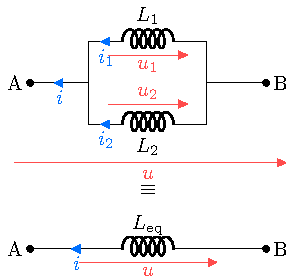
\includegraphics[width=.7\linewidth, draft=true]{bpara}
			}{
				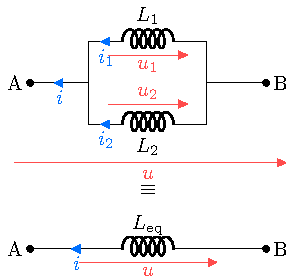
\includegraphics[width=.7\linewidth]{bpara}
			}
			\captionof{figure}{}
		\end{center}
	\end{tcb}
	\begin{tcb}[label=demo:bpara](demo)'r'{Association en parallèle}
		\psw{
			\begin{DispWithArrows*}[]
				i &= i_1+i_2
				\Arrow{$\dv{t}(~)$}
				\\\Ra
				\dv{i}{t} &= \dv{i_1}{t} + \dv{i_2}{t}
				\Arrow{$u_L = L \dv{i}{t}$}
				\\\Lra
				\frac{u}{L_{\rm eq}} &= \frac{u}{L_1} + \frac{u}{L_2}
			\end{DispWithArrows*}
			On a bien l'expression d'une unique bobine d'inductance
			\[
				\boxed{\dfrac{1}{L_{\rm eq}} = \dfrac{1}{L_1} + \dfrac{1}{L_2}}
			\]
		}
	\end{tcb}
\end{tcbraster}

\subsubsection{Bobine réelle}

\noindent
\begin{minipage}[t]{.69\linewidth}
	Dans la réalité, le fil de cuivre enroulé possède une résistance non nulle.
	Une bobine réelle se modélise donc par l’association en série d’une bobine
	idéale et d’une résistance électrique $r$.
\end{minipage}
\hfill
\begin{minipage}[t]{.30\linewidth}
	~
	\vspace{-40pt}
	\begin{center}
		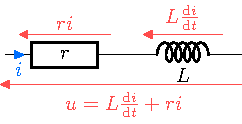
\includegraphics[width=\linewidth]{breel}
		\captionof{figure}{}
		\label{fig:breel}
	\end{center}
\end{minipage}

\subsubsection{Énergie stockée dans une bobine}
\begin{tcb}(demo)<lfnt>{}
	\textbf{En convention récepteur}, la puissance \textbf{reçue} est
	\psw{
		\begin{DispWithArrows*}
			\Pc_{L} &= u_Li
			\Arrow{$u_L = L \dv{i}{t}$}
			\\\Lra
			\Pc_{L} &= Li \dv{i}{t} \triangleq \dv{\Ec_L}{t}
		\end{DispWithArrows*}
	}
	\vspace{-15pt}
	\leftcenters{\hspace{-12pt}Or, $\forall f$ fonction dérivable,}
	{\psw{$\DS\boxed{f\times f' = \left( \frac{1}{2}f^2 \right)'}$}}
	\smallbreak
	Ainsi,
	\psw{
		\[
			\Pc_{L} = \dv{t} \left( \frac{1}{2} Li{}^2 \right)
			\Rightarrow \Ec_C(t) = \frac{1}{2}L i(t)^2
		\]
	}
	\vspace{-15pt}
\end{tcb}

\begin{tcb}[label=prop:El](prop){Énergie stockée dans une bobine}
	\psw{
		\[
			\boxed{\Ec_L(t) = \frac{1}{2}L i{}^2(t)}
		\]
	}
	\vspace{-10pt}
\end{tcb}
\begin{tcb}[label=rema:genrec, sidebyside](rema){Bobine réceptrice ou
			génératrice}
	Par l'étude de la relation précédente,
	\psw{
		\[
			i \nearrow \quad \Ra \dv{i}{t} > 0 \Rightarrow \Pc_{L} > 0
		\]
	}
	ainsi, la bobine reçoit bien de l'énergie au reste du circuit, et elle se
	\textbf{comporte comme un récepteur}.
	\tcblower
	À l'inverse, on lit que
	\psw{
		\[
			i \searrow \quad \Ra \dv{i}{t} < 0 \Rightarrow \Pc_{L} < 0
		\]
	}
	ainsi, la bobine cède en réalité de l'énergie au reste du circuit,
	autrement dit \textbf{il peut se comporter comme un générateur}~!
\end{tcb}

\subsection{Circuit RL série~: échelon montant}
\subsubsection{Présentation}
\noindent
\begin{minipage}[c]{.6\linewidth}
	\begin{itemize}
		\item Il est constitué d'un générateur idéal de tension en série avec une
		      résistance et une bobine idéale.
		\item \textbf{On suppose l'interrupteur initialement ouvert}.
		\item À $t=0$, on ferme l'interrupteur.
	\end{itemize}
\end{minipage}
\hfill
\begin{minipage}[c]{.35\linewidth}
	~
	\begin{center}
		\switch{
			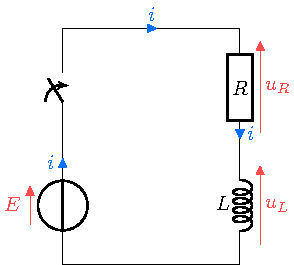
\includegraphics[width=.9\linewidth, draft=true]{circ_rl-start}
		}{
			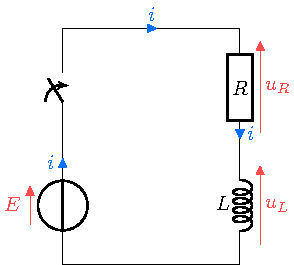
\includegraphics[width=.9\linewidth]{circ_rl-start}
		}
		\label{fig:circ_rl-start}
		\captionof{figure}{}
	\end{center}
\end{minipage}

\subsubsection{Équation différentielle du circuit}
On cherche à connaître la tension aux bornes du condensateur à partir du moment
où l’on ferme l’interrupteur, soit à $t \geq 0$.
\begin{tcb}[label=demo:eqdiffrl](demo)<lfnt>{Équa. diff. RL montant}
	Avec la loi des mailles,
	\psw{
		\begin{DispWithArrows*}
			u_L + u_R &= E
			\Arrow{$u_R = Ri$\\et $u_L = L \dv{i}{t}$}
			\\\Lra
			L \dv{i}{t} + Ri        & = E
			\\\Lra
			\dv{i}{t} + \frac{R}{L}i & = \frac{E}{L}
		\end{DispWithArrows*}
	}
	\vspace{-15pt}
\end{tcb}
\begin{tcb}[label=prop:eqdifflc, sidebyside, righthand ratio=.4](prop){Équation
			différentielle RL échelon montant}

	L'équation différentielle du courant $i(t)$ aux bornes d'une bobine
	dans un circuit RL avec un échelon de tension montant $E$ s'écrit
	\psw{
		\[
			\boxed{\dv{i}{t} + \frac{1}{\tau}i = \frac{1}{\tau}\frac{E}{R}}
		\]
	}
	avec \fbox{$\tau = L/R$} la constante de temps.
	\tcblower
	C'est une équation différentielle linéaire du premier ordre à
	coefficients et second membre constants, de condition initiale
	\psw{
		\[
			\boxed{i(0^-) = i(0^+) = 0}
		\]
	}
\end{tcb}

\begin{tcb}(rema){Unité de $L/R$}
	On peut de même démontrer l'unité de $L/R$ par analyse dimensionnelle.
\end{tcb}

\subsubsection{Résolution de l'équation différentielle}
\begin{tcb}[label=demo:rlsolu](demo){Solution RL série montant}
	\begin{enumerate}[label=\sqenumi]
		\item L'équation homogène est~:
		      \psw{
			      \[
				      \dv{i}{t} + \frac{1}{\tau}i = 0
			      \]
		      }
		      \vspace{-15pt}
		\item La forme générale de la solution pour cette équation est~:
		      \psw{
			      \[
				      i(t) = K\exp\left( -\frac{t}{\tau} \right)
			      \]
		      }
		      \vspace{-15pt}
		\item Une solution particulière avec $i(t) = \lambda$ donne
		      \psw{
			      \[
				      0 + \frac{\lambda}{\tau} = \frac{1}{\tau}\frac{E}{R}
			      \]
			      Donc $i(t) = \frac{E}{R}$ est \textbf{une} solution de l'équation
			      différentielle.
		      }
		\item La solution générale est donc
		      \psw{
			      \[
				      i(t) = \frac{E}{R} + K\exp \left( - \frac{t}{\tau} \right)
			      \]
		      }
		      \vspace{-15pt}
		\item Les conditions initiales donnent ici
		      \[
			      \psw{i(t=0) = 0}
			      \qqet
			      \psw{i(0) = K + \frac{E}{R} \Ra K=-\frac{E}{R}}
		      \]
	\end{enumerate}
\end{tcb}
\begin{tcb}[label=prop:isolu, sidebyside, righthand ratio=.4](prop){Solution
			de l'équation différentielle RL montant}
	La solution de l'équation différentielle du courant $i(t)$ d'un circuit RL
	soumis à un échelon de tension $E$ avec $i(0) = 0$ est
	\psw{
		\[
			\boxed{i(t) = \frac{E}{R}\left(1-\exp\left(-\frac{t}{\tau}\right)\right)}
		\]
	}
	\vspace{-15pt}
	\tcblower
	\begin{center}
		\switch{
			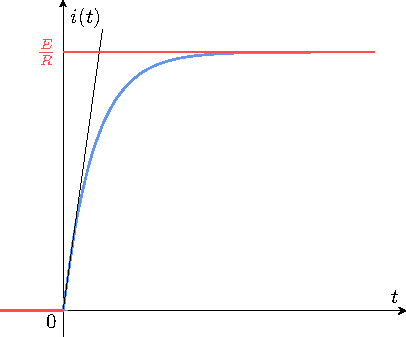
\includegraphics[width=\linewidth, draft=true]{carac_rl}
		}{
			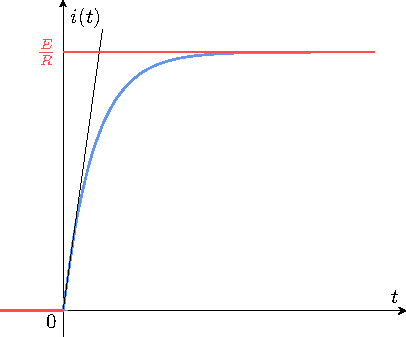
\includegraphics[width=\linewidth]{carac_rl}
		}
		\captionof{figure}{}
	\end{center}
\end{tcb}

\subsubsection{Constante de temps, régime transitoire}
\begin{tcbraster}[raster columns=2, raster equal height=rows]
	\begin{tcb}[label=impl:déterm](exem){Détermination $\tau$}
		Avec la courbe $i(t)$, on remarque que~:
		\begin{enumerate}
			\item \psw{
				      $i(\tau) = \frac{E}{R} \left( 1-e^{-1} \right) \approx
					      \num{0.632}\times E$
			      }
			      \smallbreak
			      Donc on trouve $\tau$ en lisant l'abscisse telle que $i(\tau) =
				      \num{0.632}\times \frac{E}{R}$.
			\item En $t=0$, l'équation différentielle donne
			      \psw{
				      \[
					      \dv{i}{t}\/ (0) + \underbracket[1pt]{\frac{i(0)}{\tau}}_{=0}
					      = \frac{1}{\tau}\frac{E}{R}
				      \]
			      }
			      La tangente à la courbe en 0, de pente $\frac{E}{R\tau}$ coupe donc
			      l'asymptote en $t = \tau$.
		\end{enumerate}
	\end{tcb}
	\begin{tcb}*[label=impl:tauRL](impl)"limp"'r'{Constante de temps}
		\switch{
			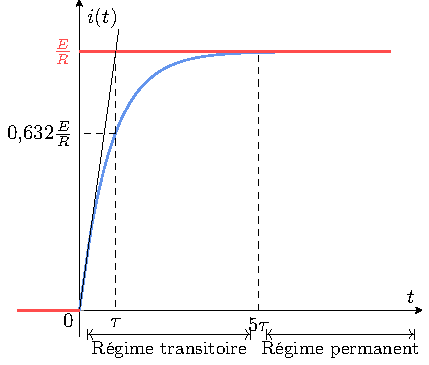
\includegraphics[width=\linewidth, draft=true]{carac_rl-tau}
		}{
			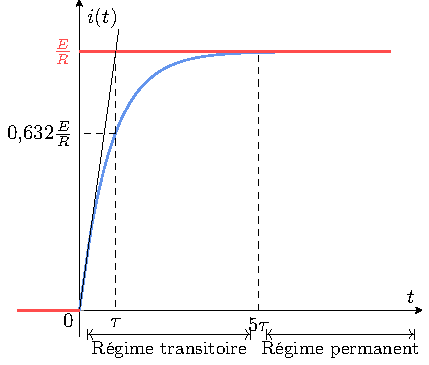
\includegraphics[width=\linewidth]{carac_rl-tau}
		}
		\captionof{figure}{}
	\end{tcb}
\end{tcbraster}

Comme précédemment, avec $t_{99}$ tel que $i(t_{99}) = \num{0.99}\frac{E}{R}$,
on trouve $t_{99} = \num{4.6}\tau$.
\begin{tcb}(prop){Temps de réponse}
	\leftcenters{Ainsi,}
	{\psw{\fbox{le temps de réponse à 99\% est à \num{4.6}$\tau$}}}
\end{tcb}

\subsubsection{Évolution de la tension}
\begin{tcb}[label=demo:url-charge](demo)<lfnt>{Tension RL charge}
	\begin{enumerate}
		\item Avec la caractéristique de L~:
		      \psw{
			      \begin{DispWithArrows*}
				      u_L(t)             & = L \dv{i}{t}
				      \Arrow{$i(t) = \frac{E}{R}(1-\exr^{-t/\tau})$}
				      \\\Ra
				      u_L(t) & = \frac{LE}{R} \left(
				      0 - \left(-\frac{1}{\tau} \right)
				      \exp \left(- \frac{t}{\tau} \right)
				      \right)
				      \Arrow{$\tau = L/R$}
				      \\\Lra
				      \Aboxed{u_L(t) &= E\exp \left(-\frac{t}{\tau} \right)}
			      \end{DispWithArrows*}
		      }
		\item Avec la loi des mailles~:
		      \psw{
			      \begin{DispWithArrows*}
				      u_L &= E - Ri
				      \Arrow{$i(t) = \frac{E}{R}(1-\exr^{-t/\tau})$}
				      \\\Lra
				      u_L(t) &= E -R \frac{E}{R}(1-\exr^{-t/\tau})
				      \\\Lra
				      \Aboxed{u_L(t) &= E\exp \left(-\frac{t}{\tau} \right)}
			      \end{DispWithArrows*}
		      }
	\end{enumerate}
\end{tcb}
\begin{tcb}[label=prop:url-charge, sidebyside, righthand ratio=.4](prop){Tension RL charge}
	La tension dans un circuit RL en charge s'exprime par
	\psw{
		\[
			\boxed{u_L(t) = E\exp \left(-\frac{t}{\tau} \right)}
		\]
	}
	\tcblower
	\begin{center}
		\switch{
			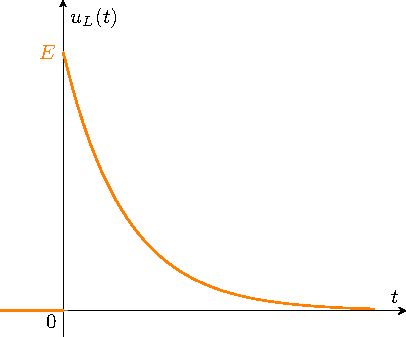
\includegraphics[width=\linewidth, draft=true]{carac_rlU}
		}{
			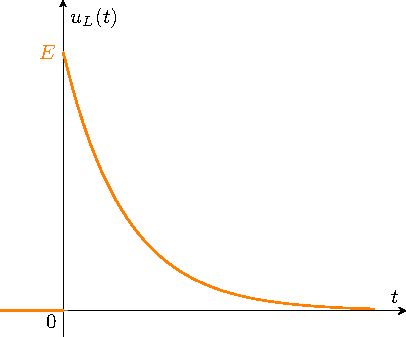
\includegraphics[width=\linewidth]{carac_rlU}
		}
		\captionof{figure}{}
	\end{center}
\end{tcb}

\subsubsection{Bilan de puissance}

\begin{tcb}[label=demo:rlpuiss-charge](demo)<lfnt>{Bilan de puissances}
	\vspace{-15pt}
	\psw{
		\begin{DispWithArrows*}
			u_L + Ri &= E
			\CArrow{$\times i$}
			\\\Lra
			u_L\,i + Ri^{2} &= Ei
			\Arrow{RCT pour L~: $u_L = L \dv{i}{t}$}
			\\\Lra
			i\,L \dv{i}{t} + Ri^{2} &= Ei
			\Arrow{$f \times f' = \left( \frac{1}{2}f^{2} \right)'$}
			\\\Lra
			\underbracket[1pt]{\dv{t} \left( \frac{1}{2}Li{}^{2} \right)}
			_{\dv{\Ec_L}{t}} +
			\underbracket[1pt]{\vphantom{\dv{t} \left( \frac{1}{2}Li{}^{2} \right)}
				Ri^{2}}_{\Pc_J}
			&=
			\underbracket[1pt]{\vphantom{\dv{t} \left( \frac{1}{2}Li{}^{2} \right)}
				Ei}_{\Pc_G}
		\end{DispWithArrows*}
	}
	\vspace{-15pt}
\end{tcb}
\begin{tcb}[label=prop:rlpuiss-charge](prop){Bilan de puissances}
	Dans un circuit RL en charge, on a le bilan de puissances
	\psw{
		\[
			\boxed{\Pc_G = \Pc_L + \Pc_J}
		\]
	}
	\vspace{-15pt}
	\begin{itemize}[leftmargin=50pt]
		\item[$\Pc_G = Ei$] : \psw{
				la puissance fournie par le générateur~;
			}
		\item[$\Pc_L = \dv{\Ec_L}{t}$] : \psw{
				la puissance reçue par le condensateur~;
			}
		\item[$\Pc_J = Ri^{2}$] : \psw{
				la puissance dissipée par effet \textsc{Joule} dans la
				résistance.
			}
	\end{itemize}
\end{tcb}

\begin{tcb}[bld, cnt](impo){Bilan de puissance RL charge}
	Ici la puissance en régime permanent n'est pas nulle~: un courant circule
	toujours dans la résistance qui dissipe $RI^2$. On ne peut intégrer à
	l'infini.
\end{tcb}

\subsection{Circuit RL série~: décharge}
\subsubsection{Présentation}
\noindent
\begin{minipage}[c]{.6\linewidth}
	\begin{itemize}
		\item Il est constitué d'un générateur idéal de tension en série avec une
		      résistance et une bobine idéale.
		\item \textbf{On suppose le courant initialement établi}~: $i(0^-) =
			      \frac{E}{R}$.
		\item À $t=0$, on coupe le générateur.
	\end{itemize}
	On dit que le système est \textbf{en régime libre} et soumis à un
	\textbf{échelon de tension descendant}.
\end{minipage}
\hfill
\begin{minipage}[c]{.35\linewidth}
	~
	\begin{center}
		\switch{
			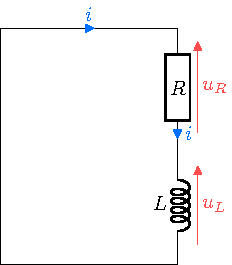
\includegraphics[width=.9\linewidth, draft=true]{circ_rl-decharge}
		}{
			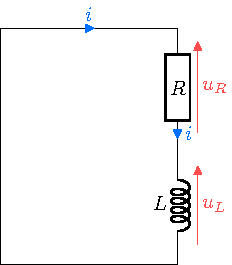
\includegraphics[width=.9\linewidth]{circ_rl-decharge}
		}
		\label{fig:circ_rl-dech}
		\captionof{figure}{}
	\end{center}
\end{minipage}

\subsubsection{Équation différentielle du circuit}
\begin{tcbraster}[raster columns=2, raster equal height=rows]
	\begin{tcb}[label=prop:eqdiffrl](prop){Équa. diff. RL libre}
		L'équation différentielle du courant $i(t)$ aux bornes d'un
		condensateur dans un circuit RL en décharge
		\psw{
			\[ \boxed{\dv{i}{t} + \frac{1}{\tau}i = 0}\]
		}
		avec \fbox{$\tau = L/R$} la constante de temps.
		\tcblower
		C'est une équation différentielle linéaire du premier ordre à
		coefficients constants sans second membre, de condition initiale
		\psw{
			\[ \boxed{i(0^-) = i(0^+) = \frac{E}{R}}\]
		}
	\end{tcb}
	\begin{tcb}[label=demo:eqdiffrl](demo)'r'{Équa. diff. RL libre}
		Avec la loi des mailles,
		\psw{
			\begin{DispWithArrows*}[fleqn, mathindent=1cm]
				u_R + u_L &= 0
				\Arrow{$u_R = Ri$\\et $u_L = L \dv{i}{t}$}
				\\\Lra
				L \dv{i}{t} + Ri        & = 0
				\\\Lra
				\dv{i}{t} + \frac{R}{L}i & = 0
			\end{DispWithArrows*}
		}
	\end{tcb}
\end{tcbraster}

\subsubsection{Résolution de l'équation différentielle}
\begin{tcbraster}[raster columns=2, raster equal height=rows]
	\begin{tcb}[label=prop:rlsoludech](prop){Solution équa. diff. RL libre}
		La solution de l'équation différentielle de la tension $i(t)$
		d'un circuit RL en décharge avec $i(0) = \frac{E}{R}$ est
		\psw{
			\[\boxed{i(t) = \frac{E}{R}\exp\left(-\frac{t}{\tau}\right)}\]
		}
	\end{tcb}
	\begin{tcb}[label=demo:rlsoludech](demo)'r'{Solution équa. diff. RL libre}
		L'équation étant déjà homogène, on écrit la forme générale~:
		\psw{
			\[i(t) = K\exp\left( -\frac{t}{\tau} \right)\]
		}
		et on trouve $K$ avec la condition initiale~:
		\[
			\psw{i(0) = \frac{E}{R}}
			\qqet
			\psw{i(0) = K \Ra K=\frac{E}{R}}
		\]
	\end{tcb}
\end{tcbraster}

\subsubsection{Représentation graphique, constante de temps et transitoire}
\begin{tcbraster}[raster columns=2, raster equal height=rows]
	\begin{tcb}[label=impl:déterm](exem){Détermination $\tau$}
		\begin{enumerate}
			\item \psw{
				      $i(\tau) = \frac{E}{R} e^{-1} \approx
					      \num{0.368}\times \frac{E}{R}$
			      }
			      \smallbreak
			      Donc on trouve $\tau$ en lisant l'abscisse telle que $i(\tau) =
				      \num{0.368}\times \frac{E}{R}$.
			\item En $t=0$, l'équation différentielle donne
			      \psw{
				      \[
					      \dv{i}{t}\/ (0) + \overbracket[1pt]{\frac{i(0)}{\tau}}^{=E/R}
					      = 0
				      \]
			      }
			      La tangente à la courbe en 0, de pente $\frac{-E}{R\tau}$ coupe
			      donc l'asymptote en $t = \tau$.
		\end{enumerate}
	\end{tcb}
	\begin{tcb}*[label=impl:tauRL](impl)"limp"'r'{Constante de temps}
		\switch{
			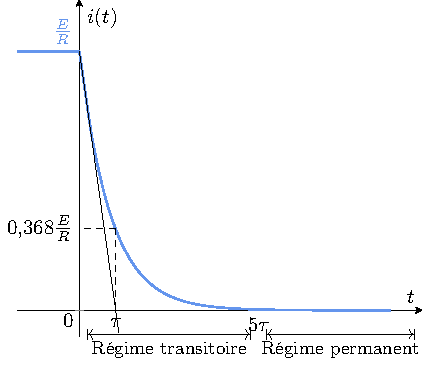
\includegraphics[width=\linewidth, draft=true]{carac_rl-tau_decharge}
		}{
			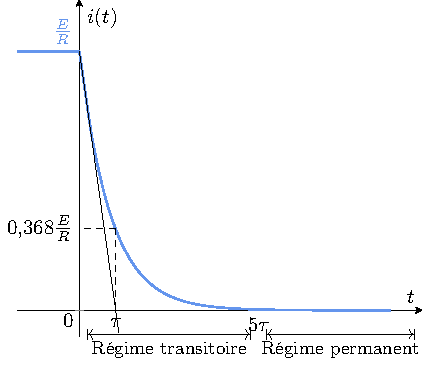
\includegraphics[width=\linewidth]{carac_rl-tau_decharge}
		}
		\captionof{figure}{}
	\end{tcb}
\end{tcbraster}
Comme précédemment, avec $t_{99}$ tel que $i(t_{99}) = \num{0.01}\frac{E}{R}$,
on trouve $t_{99} = \num{4.6}\tau$.
\begin{tcb}(prop){Temps de réponse}
	\leftcenters{Ainsi,}
	{\psw{\fbox{le temps de réponse à 99\% est à \num{4.6}$\tau$}}}
\end{tcb}

\subsubsection{Évolution de la tension}
\begin{tcb}[label=demo:irc-decharge](demo)<lfnt>{Tension RL décharge}
	\begin{enumerate}
		\item Avec la caractéristique de L~:
		      \psw{
			      \begin{DispWithArrows*}
				      u_L(t)             & = L \dv{i}{t}
				      \Arrow{$i(t) = \frac{E}{R}\exr^{-t/\tau}$}
				      \\\Ra
				      u_L(t) & = -\frac{LE}{R\tau} \exp \left(- \frac{t}{\tau} \right)
				      \Arrow{$\tau = L/R$}
				      \\\Lra
				      \Aboxed{u_L(t) &= -E\exp \left(-\frac{t}{\tau} \right)}
			      \end{DispWithArrows*}
		      }
		\item Avec la loi des mailles~:
		      \psw{
			      \begin{DispWithArrows*}
				      u_L &= - Ri
				      \Arrow{$i(t) = \frac{E}{R}\exr^{-t/\tau}$}
				      \\\Lra
				      u_L(t) &= -R \frac{E}{R}\exr^{-t/\tau}
				      \\\Lra
				      \Aboxed{u_L(t) &= -E\exp \left(-\frac{t}{\tau} \right)}
			      \end{DispWithArrows*}
		      }
	\end{enumerate}
\end{tcb}
\begin{tcb}[label=prop:url-decharge, sidebyside, righthand ratio=.4](prop){Tension RL décharge}
	La tension dans un circuit RL en décharge s'exprime par
	\psw{
		\[
			\boxed{u_L(t) = -E\exp \left(-\frac{t}{\tau} \right)}
		\]
	}
	\tcblower
	\begin{center}
		\switch{
			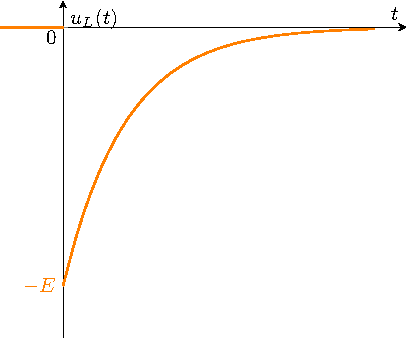
\includegraphics[width=\linewidth, draft=true]{carac_rlU_decharge}
		}{
			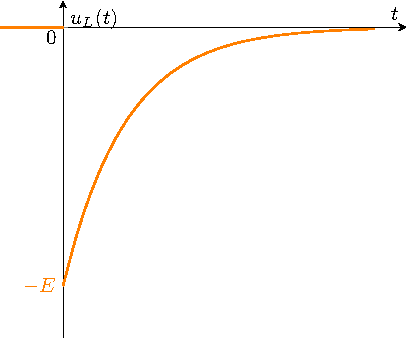
\includegraphics[width=\linewidth]{carac_rlU_decharge}
		}
		\captionof{figure}{}
	\end{center}
\end{tcb}

\end{document}
